\documentclass[11pt]{report}
\usepackage{geometry}
\usepackage{graphicx}
\usepackage{titling}
\usepackage{fancyhdr}
\usepackage{enumerate}
\usepackage{latexsym}
\usepackage{float}
\usepackage[labelfont=bf]{caption}
\usepackage[usenames,dvipsnames,svgnames,table]{xcolor}
\usepackage{listings}
\usepackage{hyperref}
\parindent=0pt
%\frenchspacing

\pagestyle{fancy}

\fancyhead[L]{\slshape\footnotesize December 9, 2014\\\textsc{02228 Fault-Tolerant Systems}}
\fancyhead[R]{\slshape\footnotesize \textsc{Andreas Kjeldsen (s092638)}\\\textsc{Morten Eskesen (s133304)}}
\fancyfoot[C]{\thepage}
\newcommand{\HRule}{\rule{\linewidth}{0.5mm}}

\begin{document}

\begin{titlepage}
\begin{center}


\includegraphics[scale=2.0]{../GFX/dtu_logo.pdf}\\[1cm]
\textsc{\LARGE Technical University of Denmark}\\[1.5cm]
\textsc{\Large 02228 Fault-Tolerant Systems}\\[0.5cm]

% Title
\HRule \\[0.4cm]
{\huge \bfseries Fault-Tolerant Cloud Computing Architectures}\\[0.1cm]
\HRule \\[1.5cm]

% Author and supervisor
{\large
\emph{Authors:} \\[10pt]
Andreas Hallberg \textsc{Kjeldsen}\\
\emph{s092638@student.dtu.dk} \\[10pt]
Morten Chabert \textsc{Eskesen}\\
\emph{s133304@student.dtu.dk}
}
\vfill

% Bottom of the page
{\large December 9, 2014}

\end{center}
\end{titlepage}

\begingroup
\tableofcontents
\let\clearpage\relax
\listoffigures
\endgroup

\chapter{Introduction}
In this report we will describe what cloud computing is, further we will give a detailed description of the architecture and fault-tolerant features of two cloud system, at last we will compare how the systems handle failures and discuss the pros and cons of these methods. As a result of the comparison, we will be able to conclude on what the systems do well and where they might be able to improve.

\section{Scope}
We will focus on the fault-tolerant features of the cloud computing architecture within the two selected cloud computing systems. We have chosen to focus on Amazon Web Services and Google Cloud Platform. We have chosen these cloud computing systems because both systems are among the most popular\footnote{Popular means that they are among the most commonly used platforms for enterprise cloud developers.} cloud computing systems \cite{cloudsurvey}.

\section{Cloud Computing}
The National Institute of Standards and Technology is a federal technology agency in the United States of America. They define cloud computing by the following:
\begin{center}
\emph{"Cloud computing is a model for enabling ubiquitous, convenient, on-demand network access to a shared pool of configurable computing resources that can be rapidly provisioned and released with minimal management effort or service provider interaction."} \cite{clouddefinition}
\end{center}
This definition states that shared networks, servers, applications, services etc can easily be distributed globally and quickly maintained by using cloud computing.\\

There are five essential characteristics of the cloud computing model
\begin{description}
\item[On-demand self-service] No required human interaction when needing more or less computing capabilities
\item[Broad network access] Capabilities are accessed through standard mechanisms and available over the network
\item[Resource pooling] Computing resources are pooled in order to serve multiple consumers 
\item[Rapid elasticity] Capabilities can be elastically released to scale rapidly according to the demand
\item[Measured service] In an automatic way the cloud computing systems control and optimize resource use
\end{description}

There are four different deployment models. One cloud infrastructure is for exclusive use by a single organization comprising the multiple consumers - the \emph{private cloud}. Another cloud infrastructure is for exclusive use by a specific community of users from organizations with shared concerns - the \emph{community cloud}. The \emph{public cloud} is an infrastructure open for use by the general public. The last cloud infrastructure is a mixture of two or more distinct cloud infrastructures that remain unique entities - the \emph{hybrid cloud}.

\section{Fault tolerance in cloud computing}
Fault tolerance is a key factor for cloud computing systems due to the rapid exponential growth in use of cloud computing \cite{faulttolerancetechniques}. The purpose of fault tolerance in any system is to achieve robustness and dependability. Fault tolerance policies and techniques allow us to classify this techniques into 2 types
\begin{description}
\item[Proactive fault tolerance policy] aims to avoid recovering from fault, errors and failure by predicting them and replacing the suspicious component. This means detecting problems before they actually occur.
\item[Reactive fault tolerance policy] reduces the effect of failures when the failure actually occurs.
\end{description}
These policies can be divided into two further sub techniques error processing and fault treatment. The aim of error processing is to remove errors from the computational state and the aim of fault treatment is to prevent faults from reoccurring.

\chapter{Amazon Web Services}
The Amazon Web Services, henceforth \emph{AWS}, is a collection of remote computing services which make up a cloud computing platform. AWS was launched by Amazon.com in 2006. This chapter will outline the architecture of their platform and describe the fault-tolerant features the platform provides.

\section{Architecture}
AWS offers a wide range of services, which can be seen as components of a system. The services they provide are available in multiple continents. The services can be used to build entire systems which are highly fault-tolerant. Using AWS the hassle of obtaining servers in various locations is removed, instead the user just has to select which region to deploy to. Though it might be tempting to just push an entire system out into the cloud, it is not enough to make it fault tolerant. The architecture of the system is important. Below is example architectures for a website and an application.

\subsection{Website architecture}
In \autoref{fig:webarchitecture} is a system with two availability zones, each hosting the web server, application server and a database server. Replication is setup between the databases. Dependencies between the availability zones has been avoided. The load balancing makes sure to distribute the traffic properly. If one of the web servers or application servers fail, then the load balancer could redirect all traffic to availability zone without errors. While the traffic is redirected, the failed instance will be replaced by instantiating a new instance from a preconfigured image.

\begin{figure}[H]
\centering
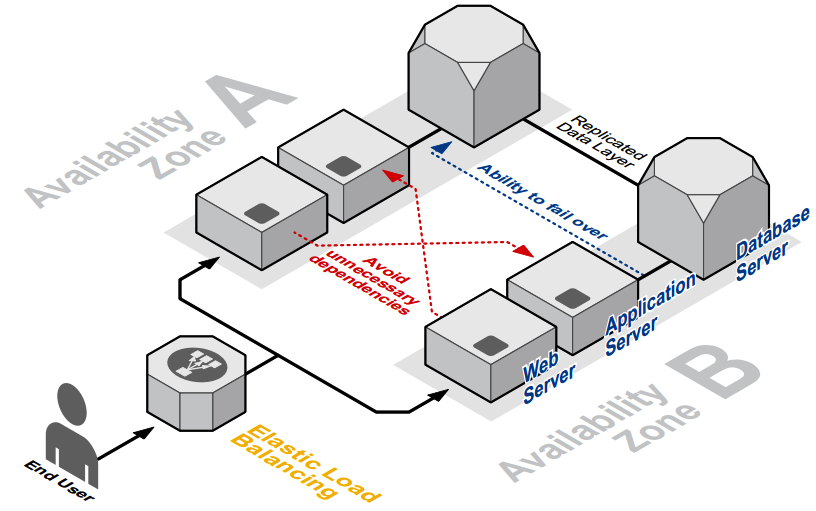
\includegraphics[scale=0.5]{../GFX/aws_architecture_web.jpg}
\caption[Example of fault-tolerant website architecture hosted on AWS]{Example of fault-tolerant website architecture hosted on AWS\cite{AWS_ac_ra_ftha_04}.}
\label{fig:webarchitecture}
\end{figure}

\subsection{Application architecture}
In \autoref{fig:apparchitecture} is a system with two availability zones, each hosting an application instance and a storage instance. At specified time intervals, snapshots of the storage instances are saved to another storage system, which also has fault-tolerance implemented. In the event of an availability zone becoming unavailable, the Elastic IP can easily be mapped to use another availability zone. In the event of an application instance crashing, the instance can easily be replaced using a preconfigured images of the instance. When the application instance has been replaced, the storage instance used is re-attached. If the storage instance fails, a new one can be instantiated from the saved snapshots.

\begin{figure}[H]
\centering
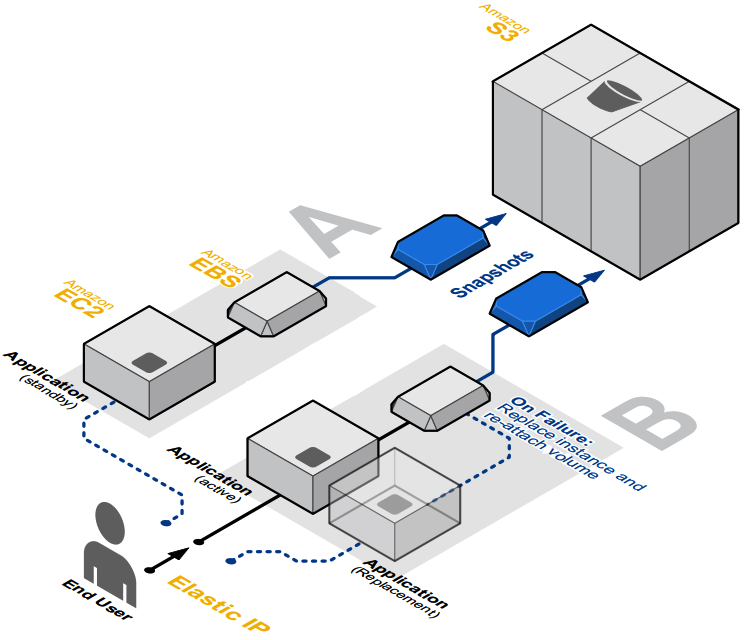
\includegraphics[scale=0.55]{../GFX/aws_architecture_app.jpg}
\caption[Example of fault-tolerant application architecture hosted on AWS]{Example of fault-tolerant application architecture hosted on AWS \cite{AWS_ac_ra_ftha_04}.}
\label{fig:apparchitecture}
\end{figure}

\section{Availability}
AWS have regions in various parts of the world. Each region has multiple Availability Zones, henceforth \emph{AZ}. When using AWS, the user has to specify in which region they wish to have their resource\footnote{A resource can be a computing resource, storage resource etc.} located. Within the region, a resource may then be distributed to multiple AZ.

\section{Redundant storage}
AWS provides multiple ways of storing data. They have key/value based storage (S3), block storage (EBS), databases (RDS, DynamoDB \& SimpleDB) and physical SSDs.

\subsection{Simple Storage Service}
The Amazon Simple Storage Service, henceforth \emph{S3}, is a highly-scalable, reliable and low-latency key/value data storage infrastructure. With S3 you define buckets in which you wish to store data. Each bucket range from 1 TB to 5TB in capacity and has a maximum file size of 5 GB. Within a region, the data stored in S3 is replicated to various AZ, hence redundancy is implemented. AWS states that S3 provides 99.999999999\% durability of a file, which means that every 10,000,000 years a file might be lost \cite{AWS_S3_FAQ}. Storing the data within various AZ, allows S3 to fetch the data requested from whichever AZ that contains the requested data with the lowest latency. Though the data is available from multiple AZ in the region, it can be setup to also be replicated to different regions, which in turn replicates the data to the various AZ in the region. The data can also be made less redundant, which means a lower cost, but only 99.99\% durability.

\subsection{Elastic Block Storage}
The Amazon Elastic Block Storage, henceforth \emph{EBS}, is block storage for use with their Elastic Compute Cloud. The blocks can be used just like an ordinary hard drive. There EBS is backed by either SSD disks or magnetic disks. It is recommended to use the SSD backed EBS for services and applications and only use the magnetic disks for data that is rarely accessed. EBS can be run in four different RAID\footnote{RAID stands for Redundant Array of Independent Disks.} configurations. The configurations are RAID0 (striped disks), RAID1 (mirroring), RAID5 (striping with distributed parity) and RAID6 (striping with double distributed parity). Amazon recommend RAID0 for use when I/O performance is more important than fault-tolerance, RAID1 when fault-tolerance is more important than I/O performance and they discourage the use of RAID5 and RAID6 \cite{AWS_raid_config}. Snapshots are created of the EBS volumes and stored on S3, thus the EBS volumes can be recreated at any time.

\subsection{Databases}
Amazon provides three types of databases. The Amazon Relational Database Service, henceforth \emph{RDS}, is a relational database service. The Amazon DynamoDB is a fully managed NoSQL database. The Amazon SimpleDB is a non-relational data store. Common for all the databases, is the way their data is stored. When data is stored in the databases it is replicated to multiple AZ and stored, which means the data is highly available and redundantly stored. RDS support snapshots, also known as DB snapshots. A DB snapshot is a point in time image of the database. DB snapshots are created in user setup intervals and have a retention period of up to 30 days. Full backups of RDS can also be made and stored on S3 to further increase the redundancy. DynamoDB and SimpleDB can be backed up manually to S3.

\subsection{SSDs}
The Amazon Elastic Compute Cloud, henceforth \emph{EC2}, are computing instances. The EC2 instances comes in various versions ranging from small instances with limited capabilities to large extravagant instances that are fully equipped. The smaller instances have no hard drive but are using EBS instead. The larger instances can both use EBS and hard drives. The hard drives used are SSDs and if more than one is attached to the instance, then they can be run in either RAID0 or RAID1. Some instances are optimized for EBS, which means that the overhead of using EBS instead of an attached SSD is very limited. All instances are able to access EBS, this is due to the hard drives attached to a computing instance are formatted when the instance is terminated, thus important long-term data should be stored on EBS \cite{AWS_instance_storage}. 

\section{Application Recovery}
At AWS, the computing instances are started by launching an Amazon Machine Image, henceforth \emph{AMI}. The AMIs are ready to deploy templates of the root volume (for example an operating system, an application server and applications), launch permissions and mapping to EBS volumes. Using AMIs it is easy to launch a new instance when server load is high or quickly recover from instance failures. The AMIs are stored on S3.

\section{Elastic Load Balancing}
The Amazon Elastic Load Balancing, is a service for distributing the load between running EC2 instances. Further it also allows for greater levels of fault-tolerance by routing traffic away from faulty EC2 instances. Elastic Load Balancing can be setup to automatically detect if EC2 instances are performing poorly or if they are dead, in this case the EC2 instance will no longer receive incoming traffic. While the traffic is being routed to other EC2 instances, the faulty EC2 instance will be replaced by a newly launched EC2 instance or a reserved EC2 instance. When the new EC2 instance is up and running, the Elastic Load Balancer can start routing traffic to it. If setup properly, the detection and replacement of faulty EC2 instances can be done automatically without the need of any manually interaction with the AWS. Elastic Load Balancing also allows for auto scaling, meaning if more computing power is required, a new EC2 instance can be launched and then the load balancer will start to even out the traffic. An example use for Elastic Load Balancing with auto scaling is shown in \autoref{fig:awsebs}. The example show two load balancers, where the first one spreads the traffic between the EC2 instances running the web server, the next load balancer spreads the traffic between the EC2 instances running the application server. Using this setup, it's possible to scale the EC2 instances asymmetrically, this is useful when only the EC2 instances running the web server is in need of more resources etc.

\begin{figure}[H]
\centering
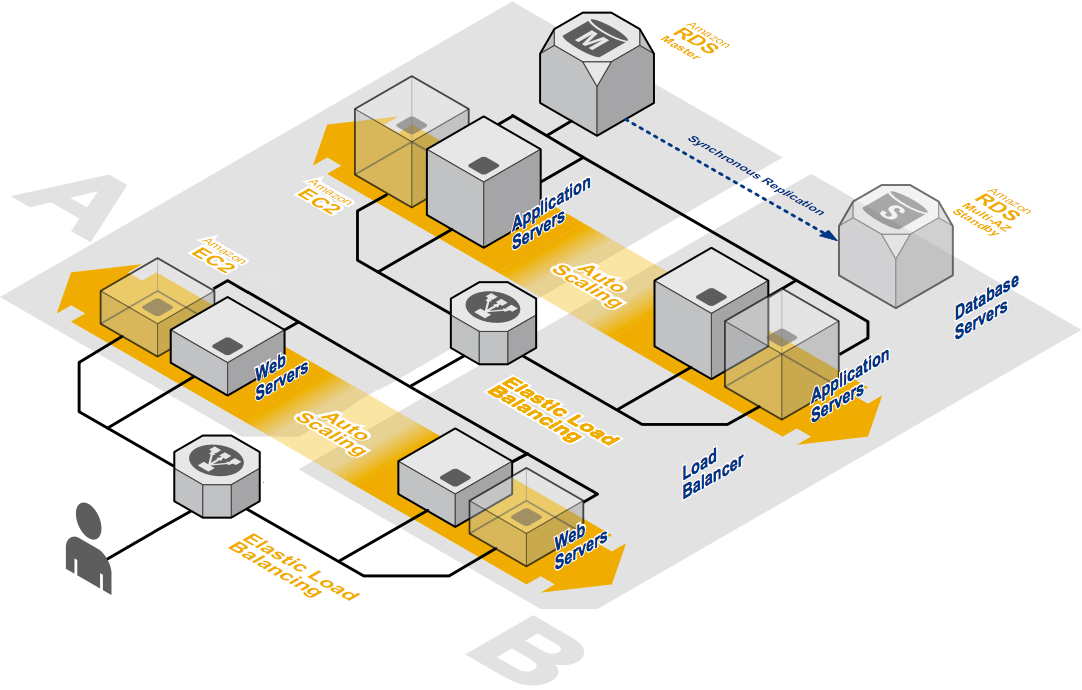
\includegraphics[scale=.38]{../GFX/aws_elb_web.jpg}
\caption{Example of using AWS Elastic Load Balancing for fault-tolerance and auto scaling.}
\label{fig:awsebs}
\end{figure}


\section{Elastic IP}
Amazon offers Elastic IP, which is a publicly accessible IP that is linked with an EC2 instance. When an EC2 instance is launched, it will get an IP assigned to it. There are no guarantee that an EC2 instance will be assigned the same IP if it has been stopped and then started again. To circumvent this problem, the Elastic IP can be used. The Elastic IP is static, hence other applications or end users will only have to access the Elastic IP and not worrying about being routed to a destination. The Elastic IP can also be used in case of an instance failure. When an instance fails, a new instance can be launched thereafter the Elastic IP is linked with the new instance. Same procedure can be applied if an availability zone becomes unavailable.


\chapter{Google Cloud Platform}
Google Cloud Platform, henceforth \emph{GCP}, is collection of cloud computing products made by Google. This chapter will outline the architecture of GCP and describe the fault-tolerant features the platform provides.

\section{Architecture}
Google App Engine, henceforth \emph{GAE}, is a service for developing and hosting web applications in Google-managed data centers. In \autoref{fig:webapparchitecture} the architecture of a web application on GAE is depicted. The Google Load Balancer makes sure to distribute the traffic properly. The load balancer is a built-in feature of GAE that provides transparent Layer 3 and Layer 7 load balancing to applications. GAE has an automatic scaling feature. When the number of request increases for an application GAE will automatically allocate more resources such that the web application is able to handle the additional demand.The Memcache and Task Queue services are integrated within GAE. The Memcache is an in-memory cache shared across all of the GAE instances. This means that there is extremely high speed access to information cached by the web-server. Task Queue provides a mechanism to free the front end servers to service new user requests by offloading longer running tasks to backend servers. Google Cloud Storage is an online storage service for files, i.e. the static content. Meanwhile the dynamic content from databases is handled by the Google Cloud SQL and Google Cloud Datastore. Google Cloud SQL is a fully managed MySQL database that lives in the Google Cloud infrastructure. Google Cloud Datastore is a fully managed, highly available NoSQL data storage for non-relational data that includes a REST API.

\begin{figure}[H]
\centering
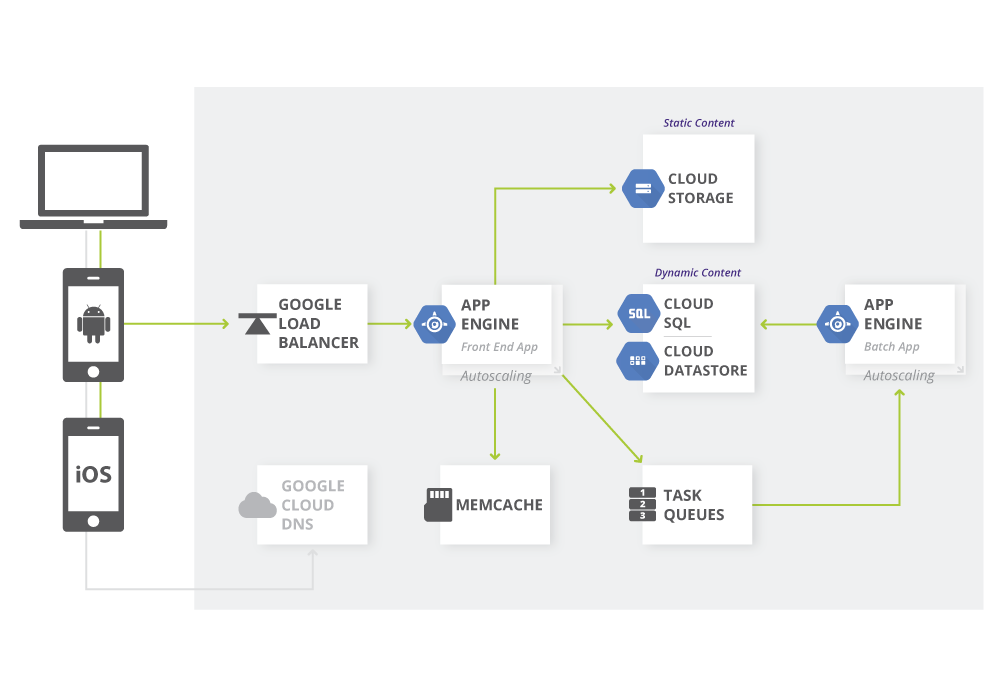
\includegraphics[scale=0.43]{../GFX/GCPwebapparchi}
\caption[Google Web Application Architecture on Google App Engine]{Google Web Application Architecture on Google App Engine \cite{google_webapp_architecture}.}
\label{fig:webapparchitecture}
\end{figure}

\section{Availability}
GCP has regions in various parts of the world. Each region has multiple availability zones. When using GCP the customer has to specify in which region their resource should be located. Only certain resources are region- and zone-specific. Resources that are specific to a zone or a region can only be used by other resources in the same zone or region. Disks and instances are examples of zonal resources. Other resources are global resources that can be used by any other resource across any location. An example of a global resource is an image. In order to build fault-tolerant applications that have high availability the recommendation from Google is to deploy applications across multiple zones in a region. The goal of this is to protect against unexpected failures of components, up to and including a single zone. When putting resources in different zones in a region it provides isolation for many types of infrastructure, hardware and software failures. Even higher degree of failure independence is achieved by putting resources in different regions.

\section{Redundant storage}
GCP provides multiple ways of storing data. They have storage for files (CS), NoSQL data storage (CD) and MySQL database (CSQL). These ways of storing data will explained in this section.

\subsection{Cloud Storage}
The Google Cloud Storage, henceforth \emph{CS}, is an online file storage web service for storing and accessing your data on Google's infrastructure. All data in CS belongs inside a project. Project consists of a set of users, a set of APIs, billing, authentication and monitoring settings for those APIs. Buckets are the basic containers that holds the data. Everything stored in CS must be contained in a bucket. Buckets belong to a project. Objects are the individual pieces of data stored in CS. The data in CS is protected through redundant storage at multiple physical locations. CS is also highly available through a fully featured API. CS provides a set of features and capabilities which are designed to store, share and manage data in an efficient and reliable way. CS also has a storage policy, that makes the stored data less durable and less available, but lower the costs of storage. It is recommended to only use the less strict storage policy for non-critical data.

\begin{description}
\item[High capability and Scalability] CS is able to store objects that are terabytes in size.
\item[Strong Data Consistency] CS provides strong read-after-write consistency for all upload and delete operations. In availability terms upload operations to CS are atomic, i.e. when uploading an object it is not accessible until it is completely uploaded.
\item[Bucket Locations] CS provides users with the ability to specify where the buckets are geographically stored.
\item[REST APIs] CS provides two RESTful programming interfaces.
\end{description}

\subsection{Cloud Datastore}
The Google Cloud Datastore, henceforth \emph{CD}, is a schemaless NoSQL datastore providing robust, scalable storage for applications. CD has the following features

\begin{itemize}
\item No planned downtime
\item Atomic transactions
\item High availability of reads and writes
\item Strong consistency for reads and ancestor queries
\item Eventual consistency for all other queries
\end{itemize}

CD replicates data across many datacenters using a system which is based on Paxos algorithm. Paxos is a family of protocols for solving consensus in a network of unreliable processors. Consensus is the process of agreeing on one result among a group of participants. Google has used the algorithm to build a fault-tolerant database, i.e. CD. CD can execute multiple operations in a single transaction. A transaction can not succeed unless every operation in the transaction succeeds. If one of the operations fail the transaction is automatically rolled back.

\subsection{Cloud SQL}
The Google Cloud SQL, henceforth \emph{CSQL}, is a MySQL database that lives in Google's cloud. It has all the capability and functionality of MySQL with a few additional features and a few unsupported features. According to Google, CSQL is ideal to use in a small to medium-sized application. CSQL offers fully managed, highly available relational databases. It is possible to create, configure and use MySQL databases that live in Google's cloud. Google handles the replication, encryption, patch management and backups. All the data is encrypted when stored and in flight on Google's network. Only authorized IP addresses are accepted when connecting to instances and can be secured with SSL. All the data is replicated in multiple locations to achieve durability and high availability.

\section{Load balancing}
Load balancing is a service for distributing the load across multiple virtual machine instances. Google Compute Engine, henceforth \emph{GCE}, is the service that allows users to launch virtual machine instances. The load balancing can be done with either network load balancing or HTTP load balancing. The load balancing provides the following benefits:

\begin{itemize}
\item Scaling of application
\item Supporting heavy traffic
\item Detection of faulty virtual machines
\item Balance load across regions
\item Route traffic to closest virtual machine
\item Support content-based routing
\end{itemize}

This means that faulty virtual machines will not cause downtime of an application as the traffic can be routed to other healthy running virtual machines or a new virtual machine can be launched to replace the faulty one. The scaling of application is done by launching new virtual machines if in need of computing power due to heavy traffic. When launching new virtual machines the load balancer will distribute the load in a way such that the traffic for each virtual machine is even.

\chapter{Comparison of Failure Handling}
In this section we will compare the fault tolerant features of Amazon Web Services and Google Cloud Platform. We will discuss their similarities and differences, while pinpointing what failure the fault-tolerant feature is to prevent.

\section{Architecture}
Both platforms consists of smaller components put together to built larger systems. They have components for computing, storage, load balancing and more. Both platforms only requires that the user should be able to architect a higher level system, meaning they should be aware of the components to use, i.e. a computing component, a file storage component and a database storage component. The platforms will then do the lower level management based on the high level architecture. This greatly increases the possibilities for users with less expertise, as they can now have scalable systems with fault tolerance while outsourcing the monitoring tasks to the platform providers. The platforms make it easy to introduce redundancy, fail-over and load balancing. Providing easy to architect fault-tolerant systems, is beneficial to both the system owners and end users. It's common for systems to provide Service Level Agreements for their end users, agreeing to have 99.9\% uptime, secure storage of their data and so forth. When building the system on a platform like AWS and GCP, the agreements can be easier to satisfy as the platforms supply the required functionality for maintaining high availability and proper storage etc. 

\subsection{Single Point of Failure}
If a system can become unavailable due to a single component, it is said to be a system with a single point of failure. The failing component causing the system to become unavailable, can be any critical component that is not being run redundantly. In both AWS and GCP, the single point of failure can easily be avoided, in fact the platforms take care of this problem automatically for some of their components. These components include but are not limited to, their file storage services and their database storage services. On the other hand they also provide components, that when not used and configured properly, can become the single point of failure. An example of this is the load balancer. If not configured to be backed by a DNS server\footnote{The DNS server is assumed to be fault-tolerant and is therefore not seen as a possible single point of failure.} that automatically detects failures and reroutes traffic, a crashed load balancer could result in an unavailable system. In general, the way to overcome single point of failure, is by using redundancy.

\section{Availability}
Both platforms are based on having regions in various parts of the world. Each region covers a large geographical area. Both platforms have multiple availability zones within their regions. The platforms differs a bit when it comes to distributing resources within a region. AWS distributes their resources to many of their availability zones, but not all. AWS supports distributing of a resources to all availability zones and regions, though this comes at an additional cost. AWS Also supports a less redundant storage option, which comes at a lower cost. GCP distributes their resources to all of their availability zones and some resources are even distributed to all regions. GCP also supports another storage method which is less durable and available, though this storage has to be actively selected. The difference in default setup comes down to whether the user has to opt-in or opt-out of higher availability and higher durability.

\subsection{Data Center Unavailability}
A system can become unavailable due to many things. One reason could be a power outage in a zone or region. If a zone becomes unavailable, most components provided by the platforms have been replicated to other availability zones and can be utilized instead. Some components, the file storage services etc, even support two zones to become unavailable at the same time. In the highly unlikely event, that 3 or more, availability zones would become unavailable at the same time, it is important to have the components of a system distributed to multiple regions. A rule of thumb is to have a redundant setup within the region and have the setup replicated to at least one other region, where it can either run in parallel or be ready to take over is necessary.

\section{Redundant Storage}
Both platforms have an online file storage web service that uses the concept of a bucket for storing files which are organized using key/value pairs. AWS' service is called S3 and GCP has CS. Both have buckets that can be terabytes in size. S3 supports files up to 5 gigabytes in size, where CS can store files that are terabytes in size. The file storage services can replicate data across multiple regions and zones within a region. Non-critical data can be stored with a less strict storage policy such that the cost of storing is lowered. The data can be stored in these services to be highly-scalable, highly available and have a high durability of the files. S3 provides durability of the files such that every 10,000,000 years at most one file might be lost. AWS offer another form of physical storage called EBS meanwhile GCP only has CS. Both platforms have databases to store dynamic content where all the data is replicated in multiple locations to achieve durability and high availability. They use the same kind of databases. GCP has no ability to store a full backup of their database on their online file storage web service whereas AWS has the ability to do a full backup of one of their databases to S3 and the ability to do a manual backup of the other two databases to S3. This further increases the redundancy for AWS.

\subsection{Data loss}
Data loss can be critical for any application. Data loss can never be fully prevented but both AWS and GCP do as much as possible to avoid the loss of data by replicating all data and storing it across multiple regions and zones. This makes it highly unlikely that data is lost by power outages, hardware faults and such in a zone or even within a region unless it happens at all the multiple locations the data is stored at. However should the data loss happen AWS has the ability to use a full backup of their databases stored in S3 to recover whereas GCP has no functionality to support this. This could be a possible improvement for GCP.

\section{Load Balancing}
Both platforms provides the possibility of using load balancing. On both platforms, the load balancer can provide more functionality than just balancing the incoming traffic. The load balancer can identify unavailable computing instances and stop sending traffic to it, further it can also instantiate a new instance if required and automatically create new instances if the load is high.

\subsection{Overload \& Crashing}
Large amount of traffic can cause an overload on the computing instances, databases and storage servers. Distributing the load between all possible instances, evens out the load, thereby decreasing response times. But sometimes, even load balancing isn't enough, not even by creating more computing instances, can the load be handled. This could occur if the system is under a Denial of Service attack. 


\chapter{Conclusion}
In this report the cloud computing platforms Amazon Web Services and Google Cloud Platform have been outlined with regards to architecture, availability, redundant storage and load balancing with focus on the fault tolerant features provided by the platform. Both platforms consists of smaller components put together to built larger systems with components for computing, storage, load balancing and more. A single point of failure can easily be avoided by both platforms, the problem is in fact taken care of automatically for some of their components. The platforms make their data centers highly available by replicating components to regions around the world, where each region have multiple availability zones. Data is replicated across these multiple regions and multiple zones within a region as well which makes it highly unlikely that data loss will become an issue when using these platforms. However Amazon Web Services have the ability to make a full backup of their databases to recover from whereas Google Cloud Platform does not which could be a possible future improvement. The report has therefore shown that the two platform use more or less the same approach for building a fault tolerant system.

\begin{thebibliography}{99}

\bibitem{AWS_ac_ra_ftha_04}
	Amazon Web Services Reference Architectures, \emph{Fault Tolerance \& High Availability}, viewed October 2014.
	\url{http://media.amazonwebservices.com/architecturecenter/AWS_ac_ra_ftha_04.pdf}
	
\bibitem{AWS_building_fault_tolerant_applications}
	Amazon Web Services Whitepapers, \emph{Building Fault Tolerant Applications}, October 2011.
	\url{http://media.amazonwebservices.com/AWS_Building_Fault_Tolerant_Applications.pdf}
	
\bibitem{AWS_slideshare_designing_fault_tolerant_applications}
	Amazon Web Services, \emph{Designing Fault-Tolerant Applications}, Slides, July 2011.
	\url{http://www.slideshare.net/AmazonWebServices/base-camp-awsdesigningfaulttolerantapplications}
	
\bibitem{AWS_youtube_designing_fault_tolerant_applications}
	Amazon Web Services, \emph{Designing Fault-Tolerant Applications}, YouTube, July 2011.
	\url{https://www.youtube.com/watch?v=9BrmHoyFJUY}

\bibitem{AWS_S3}
	Amazon Web Services, \emph{Amazon S3}, viewed October 2014.
	\url{http://aws.amazon.com/s3/}
	
\bibitem{AWS_S3_FAQ}
	Amazon Web Services, \emph{Amazon S3 FAQ}, viewed November 2014.
	\url{http://aws.amazon.com/s3/faqs/}
	
\bibitem{AWS_EBS}
	Amazon Web Services, \emph{Amazon EBS}, viewed October 2014.
	\url{http://aws.amazon.com/ebs/}
	
\bibitem{AWS_RDS}
	Amazon Web Services, \emph{Amazon RDS}, viewed October 2014.
	\url{http://aws.amazon.com/rds/}
	
\bibitem{AWS_dynamo_db}
	Amazon Web Services, \emph{Amazon DynamoDB}, viewed October 2014.
	\url{http://aws.amazon.com/dynamodb/}
	
\bibitem{AWS_simple_db}
	Amazon Web Services, \emph{Amazon SimpleDB}, viewed October 2014.
	\url{http://aws.amazon.com/simpledb/}	

\bibitem{AWS_raid_config}
	Amazon Web Services, \emph{RAID Configuration}, viewed October 2014.
	\url{http://docs.aws.amazon.com/AWSEC2/latest/UserGuide/raid-config.html}
	
\bibitem{AWS_instance_storage}
	Amazon Web Services, \emph{Instance Storage}, viewed October 2014.
	\url{http://docs.aws.amazon.com/AWSEC2/latest/UserGuide/InstanceStorage.html}

\bibitem{google_cloud_platform_documentation}
	Google, \emph{Google Cloud Platform Documentation}.
	\url{https://cloud.google.com/docs/}	
	
\bibitem{google_dataplace_for_fault_tolerance}
	Google Patents, \emph{Data placement for fault tolerance}, February 2006.
	\url{http://www.google.com/patents/US7000141}
	
\bibitem{google_webapp_architecture}
	Google Cloud Platform, \emph{Architecture: Web Application on Google App Engine}
	\url{https://cloud.google.com/solutions/architecture/webapp?hl=da}
	
\bibitem{}
	Google Cloud Docs, \emph{Regions \& Zones}
	\url{https://cloud.google.com/compute/docs/zones}
	
\bibitem{google_app_engine_scalability_2009}
	Google I/O, \emph{App Engine: Scalability, Fault Tolerance, and Integrating Amazon EC2}, YouTube, June 2006.
	\url{https://www.youtube.com/watch?v=p4F62q1kJ7I}
	
\bibitem{google_cloud_platform_blog}
	Google, \emph{Google Cloud Platform Blog}.
	\url{http://googlecloudplatform.blogspot.dk/}
	
\bibitem{google_cloud_platform_gets_developer_enhancements}
	Todd R. Weiss, \emph{Google Cloud Platform Gets Developer Enhancements}, August 2013.
	\url{http://www.eweek.com/cloud/google-cloud-platform-gets-developer-enhancements}
	
\bibitem{cloudsurvey}
	Larry Dignan, \emph{Amazon Web Services, Windows Azure top cloud dev choices, says survey}, August 2013.
	\url{http://zd.net/1vw5pzE}
	
\bibitem{clouddefinition}
	National Institute of Standards and Technology, \emph{The NIST Definition of Cloud Computing}, October 2011.
	\url{http://csrc.nist.gov/publications/nistpubs/800-145/SP800-145.pdf}
	
\bibitem{faulttolerancetechniques}
	Prasenjit Kumar Patra, Harshpreet Singh and Gurpreet Singh, \emph{Fault Tolerance Techniques and Comparative Implementation in Cloud Computing}, February 2013.
	International Journal of Computer Applications.
	
\bibitem{healthcare}
	Terrell Herzig et al., \emph{Implementing Information Security in Healthcare: Building a Security Program}, HIMSS, February 2013

\end{thebibliography}

\end{document}
